\documentclass[DaoFP]{subfiles}
\begin{document}
\setcounter{chapter}{16}

\chapter{余单子(Comonads)}

如果这个词容易发音,我们或许应该将副作用称为"ntext",因为副作用的对偶是"上下文"。

就像我们使用Kleisli箭头来处理副作用一样,我们使用co-Kleisli箭头来处理上下文。

让我们从熟悉的例子开始,将环境作为上下文。我们之前通过柯里化箭头构造了一个读取器单子(reader monad):
\begin{haskell}
(a, e) -> b
\end{haskell}
然而,这次我们将它视为一个co-Kleisli箭头,它是一个从"上下文化"参数出发的箭头。

与单子的情况类似,我们希望能够组合这样的箭头。对于携带环境的箭头来说,这相对容易:
\begin{haskell}
composeWithEnv :: ((b, e) -> c) -> ((a, e) -> b) -> ((a, e) -> c)
composeWithEnv g f = \(a, e) -> g (f (a, e), e)
\end{haskell}

实现一个关于这种组合的恒等箭头也很直接:

\begin{haskell}
idWithEnv :: (a, e) -> a
idWithEnv (a, e) = a
\end{haskell}

这强烈暗示了一个想法,即存在一个范畴,其中co-Kleisli箭头作为态射。

\begin{exercise}
证明使用\hask{composeWithEnv}组合co-Kleisli箭头是结合的。
\end{exercise}

\section{编程中的余单子}

一个函子\hask{w}(可以将其视为一个风格化的倒置\hask{m})如果支持co-Kleisli箭头的组合,那么它就是一个余单子:

\begin{haskell}
class Functor w => Comonad w where
   (=<=) :: (w b -> c) -> (w a -> b) -> (w a -> c)
   extract :: w a -> a
\end{haskell}
在这里,组合以中缀运算符的形式书写。组合的单位称为\hask{extract},因为它从上下文中提取一个值。

让我们用我们的例子来尝试一下。将环境作为对的第一部分传递是很方便的。余单子由对构造器\hask{((,) e)}的部分应用给出的函子给出。
\begin{haskell}
instance Comonad ((,) e) where
  g =<= f = \ea -> g (fst ea, f ea)
  extract = snd
\end{haskell}

与单子一样,co-Kleisli组合可以用于无点编程风格。但我们也可以使用\hask{join}的对偶\hask{duplicate}:
\begin{haskell}
  duplicate :: w a -> w (w a)
\end{haskell}
或者称为\hask{extend}的bind的对偶:
\begin{haskell}
  extend :: (w a -> b) -> w a -> w b
\end{haskell}
以下是我们如何用\hask{duplicate}和\hask{fmap}实现co-Kleisli组合:
\begin{haskell}
   g =<= f = g . fmap f . duplicate
\end{haskell}
\begin{exercise}
用\hask{extend}实现\hask{duplicate},反之亦然。
\end{exercise}
\subsection{\hask{Stream}余单子}
余单子的有趣例子涉及更大的,有时是无限的上下文。这里有一个无限流:
\begin{haskell}
data Stream a = Cons a (Stream a)
    deriving Functor
\end{haskell}

如果我们认为这样的流是类型\hask{a}在无限尾部的上下文中的值,我们可以为它提供一个\hask{Comonad}实例:
\begin{haskell}
instance Comonad Stream where
  extract (Cons a as) = a
  duplicate (Cons a as) = Cons (Cons a as) (duplicate as)
\end{haskell}
在这里,\hask{extract}返回流的头部,\hask{duplicate}将流转换为流的流,其中每个连续的流是前一个流的尾部。

直觉是\hask{duplicate}为迭代设置了舞台,但它以一种非常通用的方式完成。每个子流的头部可以解释为原始流中未来的"当前位置"。

很容易执行一个遍历这些流的头部元素的计算。但这并不是余单子的力量所在。它让我们执行需要任意前瞻的计算。这样的计算不仅需要访问连续子流的头部,还需要访问它们的尾部。

这就是\hask{extend}所做的:它将给定的co-Kleisli箭头\hask{f}应用于\hask{duplicate}生成的所有流:
\begin{haskell}
  extend f (Cons a as) = Cons (f (Cons a as)) (extend f as)
\end{haskell}

这是一个co-Kleisli箭头的例子,它计算流的前五个元素的平均值:
\begin{haskell}
avg :: Stream Double -> Double
avg  = (/5). sum . stmTake 5
\end{haskell}
它使用一个辅助函数提取前\hask{n}项:
\begin{haskell}
stmTake :: Int -> Stream a -> [a]
stmTake 0 _ = []
stmTake n (Cons a as) = a : stmTake (n - 1) as
\end{haskell}

我们可以使用\hask{extend}在整个流上运行\hask{avg}以平滑局部波动。电气工程师可能会将其识别为一个简单的\index{低通滤波器}低通滤波器,其中\hask{extend}实现了\index{卷积}卷积。它生成原始流的运行平均值。
\begin{haskell}
smooth :: Stream Double -> Stream Double
smooth = extend avg
\end{haskell}

余单子对于在空间或时间上扩展的数据结构中结构化计算非常有用。这些计算足够局部以定义"当前位置",但需要从相邻位置收集信息。信号处理或图像处理是很好的例子。模拟也是如此,其中微分方程必须在体积内迭代求解:气候模拟、宇宙学模型或核反应,仅举几例。康威的生命游戏也是测试余单子方法的好地方。

有时,在连续数据流上进行计算,直到最后一步才进行采样是很方便的。这是一个时间函数(由\hask{Double}表示)的信号示例
\begin{haskell}
data Signal a = Sig (Double -> a) Double
\end{haskell}
第一个组件是作为时间函数实现的\hask{a}的连续流。第二个组件是当前时间。

这是连续流的\hask{Comonad}实例:
\begin{haskell}
instance Comonad Signal where
  extract (Sig f x) = f x
  duplicate (Sig f x) = Sig (\y -> Sig f (x - y)) x
  extend g (Sig f x) = Sig (\y -> g (Sig f (x - y))) x
\end{haskell}
在这里,\hask{extend}将滤波器
\begin{haskell}
g :: Signal a -> a
\end{haskell}
卷积到整个流上。

\begin{exercise}
为双向流实现\hask{Comonad}实例:
\begin{haskell}
data BiStream a = BStr [a] [a]
\end{haskell}
假设两个列表都是无限的。提示:将第一个列表视为过去(按相反顺序);第二个列表的头部视为现在,其尾部视为未来。
\end{exercise}

\begin{exercise}
为上一个练习中的\hask{BiStream}实现一个低通滤波器。它对三个值进行平均:当前值、紧邻过去的值和紧邻未来的值。对于电气工程师:实现一个高斯滤波器。
\end{exercise}

\section{余单子的范畴定义}

我们可以通过反转单子定义中的箭头来得到余单子的定义。我们的 \hask{duplicate} 对应于反转的 \hask{join},而 \hask{extract} 则是反转的 \hask{return}。

因此,余单子是一个自函子 $W$,配备有两个自然变换:
\begin{align*}
\delta &\colon W \to W \circ W \\
\varepsilon &\colon W \to \text{Id} 
\end{align*}

这些变换(分别对应于 \hask{duplicate} 和 \hask{extract})必须满足与单子相同的恒等式,只是箭头方向相反。

以下是余单位律:
\[
 \begin{tikzcd}
\text{Id} \circ W
 \arrow[rrd, "="']
& & W \circ W
 \arrow[ll, "\varepsilon \circ W"']
 \arrow[rr, "W \circ \varepsilon"]
&& W \circ \text{Id}
 \arrow[lld, "="]
 \\
 && W
  \arrow[u, "\delta"]
 \end{tikzcd}
\]
以及结合律:
\[
 \begin{tikzcd}
 (W \circ W) \circ W 
 \arrow[rr, "="]
 &&
 W \circ (W \circ W)
 \\
 W \circ W 
 \arrow[u, "\delta \circ W"]
& & W \circ W
 \arrow[u, "W \circ \delta"']
 \\
&  W
 \arrow[ul, "\delta"]
 \arrow[ur, "\delta"']
 \end{tikzcd}
\]

\subsection{余幺半群}

我们已经看到单子定律如何从幺半群定律中得出。我们可以预期余单子定律应该从幺半群的对偶版本中得出。

事实上,\index{余幺半群}\emph{余幺半群} 是幺半群范畴 $(\mathcal{C}, \otimes, I)$ 中的一个对象 $w$,配备有两个称为余乘法和余单位的态射:
\begin{align*}
\delta &\colon w \to w \otimes w \\
\varepsilon &\colon w \to I
\end{align*}
我们可以将张量积替换为自函子的复合,将单位对象替换为恒等函子,从而将余单子定义为自函子范畴中的余幺半群。

在 Haskell 中,我们可以为笛卡尔积定义一个 \hask{Comonoid} 类型类:
\begin{haskell}
class Comonoid w where
  split   :: w -> (w, w)
  destroy :: w -> ()
\end{haskell}

余幺半群比其兄弟幺半群讨论得少,主要是因为它们被视为理所当然。在笛卡尔范畴中,每个对象都可以通过使用对角映射 $\Delta_a \colon a \to a \times a$ 作为余乘法,以及到终端对象的唯一箭头作为余单位,来变成一个余幺半群。

在编程中,这是我们不假思索就会做的事情。余乘法意味着能够复制一个值,而余单位意味着能够丢弃一个值。

在 Haskell 中,我们可以轻松地为任何类型实现 \hask{Comonoid} 实例:
\begin{haskell}
instance Comonoid w where
  split w   = (w, w)
  destroy w = ()
\end{haskell}
事实上,我们不会多想就使用一个函数的参数两次,或者根本不使用它。但是,如果我们想要明确表达,像这样的函数:
\begin{haskell}
f x = x + x
g y = 42
\end{haskell}
可以写成:
\begin{haskell}
f x = let (x1, x2) = split x 
      in x1 + x2
g y = let () = destroy y 
      in 42
\end{haskell}

然而,在某些情况下,复制或丢弃一个变量是不可取的。这种情况通常发生在参数是外部资源时,比如文件句柄、网络端口或堆上分配的一块内存。这些资源在被分配和释放之间应该有明确的生命周期。跟踪可以轻松复制或丢弃的对象的生命周期非常困难,并且是编程错误的常见来源。

基于笛卡尔范畴的编程模型总是会有这个问题。解决方案是使用不支持对象复制或销毁的幺半群(闭)范畴。这样的范畴是 \index{线性类型}\emph{线性类型} 的自然设置。线性类型的元素在 \index{Rust}Rust 中使用,并且在撰写本文时,正在 Haskell 中进行尝试。在 C++ 中,有一些构造模仿线性性,比如 \hask{unique_ptr} 和移动语义。

\section{伴随函子导出的余单子}

我们已经看到,两个函子 $L \colon \mathcal{D} \to \mathcal{C}$ 和 $R \colon \mathcal{C} \to \mathcal{D}$ 之间的伴随关系 $L \dashv R$ 会导出一个单子 $R \circ L \colon \mathcal{D} \to \mathcal{D}$。另一种组合 $L \circ R$ 是 $\mathcal{C}$ 上的自函子,它实际上是一个余单子。

伴随关系的余单位(counit)充当了余单子的余单位。这可以通过以下字符串图来说明:
\[
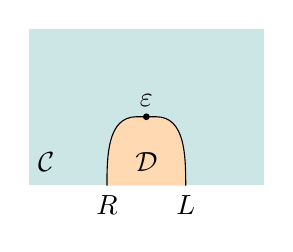
\begin{tikzpicture}
\def\xleft{0.5};
\def\xmid{1};
\def\xright{1.5};

\def \ybot{0};
\def \ymid{1};
\def \ytop{2 * \ymid};
%\def \yt{2 * \ymid - 0.3};
\def \yb{2 * \ybot + 0.3};

\node [below] (a) at (\xleft, \ybot) {$R$};
\node(b) [below] at (\xmid, \ymid) {};
\node[below] (c) at (\xright, \ybot) {$L$};

\filldraw[fill=blue!50!green!20, draw=white] (\xleft-1, \ytop) rectangle (\xright+1, \ybot);

\draw [fill=orange!30] (a.north) to [out=90, in=180] (b.west) -- (b.east) to [out=0, in=90] (c.north);

\filldraw[black] (b) circle (1 pt);
\node [above] at (b) {$\varepsilon$};

\node(l)[right] at (\xleft-1, \yb) {$\mathcal{C}$};
\node(r) at (\xmid, \yb) {$\mathcal{D}$};

\end{tikzpicture}
\]

余乘法(comultiplication)由 $\eta$ 的whiskering给出:
\[ \delta = L  \circ \eta \circ R \]
如下字符串图所示:
\[
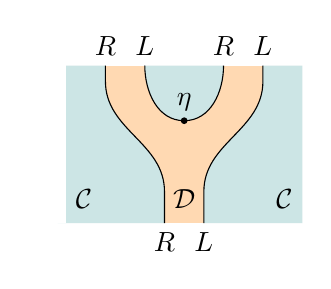
\begin{tikzpicture}
\def \xmid          {0};
\def \xr               {0.5};
\def \xrr             {1}
\def \xrm            {0.25}
\def \xrightmost {1.5}
\def \xl {-\xr}
\def \xll {-\xrr}
\def \xlm {-\xrm}
\def \xleftmost {-\xrightmost}

\def \ybot           {0};
\def \ymidbot     {-0.20};
\def \yeps          {-0.7};
\def \ymid          {-1};
\def \ymidtop     {-1.60}
\def \ytop           {-2};
\def \ylabel        {\ytop + 0.3};
% functors
\node [below] at (\xlm, \ytop)  {$R$};
\node [below] at (\xrm, \ytop) {$L$};

\node [above] at (\xll, \ybot) {$R$};
\node [above] at (\xl, \ybot) {$L$};
\node [above] at (\xr, \ybot) {$R$};
\node [above] at (\xrr, \ybot) {$L$};

\filldraw[fill=orange!30, draw=white] (\xleftmost, \ytop) rectangle (\xrightmost, \ybot);

% left area
\path [fill=blue!50!green!20] (\xleftmost, \ybot) to  (\xll, \ybot) to (\xll, \ymidbot) [out=-90, in=90] to (\xlm, \ymidtop) to  (\xlm, \ytop) to [out=180, in=180] (\xleftmost, \ytop);
% right area
\path [fill=blue!50!green!20] (\xrightmost, \ybot) to (\xrr, \ybot) to (\xrr, \ymidbot) [out=-90, in=90] to (\xrm, \ymidtop) to (\xrm, \ytop) to [out=0, in=180]  (\xrightmost, \ytop);
% cap
\draw [fill=blue!50!green!20] (\xl, \ybot) to [out=-90, in=180] (\xmid, \yeps) to [out=0, in=-90] (\xr, \ybot);
% left curve
\draw (\xll, \ybot) to (\xll, \ymidbot) [out=-90, in=90] to (\xlm, \ymidtop) to  (\xlm, \ytop);
% right curve
\draw (\xrr, \ybot) to (\xrr, \ymidbot) [out=-90, in=90] to (\xrm, \ymidtop) to (\xrm, \ytop);
% eta
\filldraw [black] (\xmid, \yeps) circle (1 pt);
\node [above] at (\xmid, \yeps) {$\eta$};
% categories
\node [right] at (\xleftmost, \ylabel) {$\mathcal{C}$};
\node           at (\xmid, \ylabel)        {$\mathcal{D}$};
\node [left]   at (\xrightmost, \ylabel) {$\mathcal{C}$};

\end{tikzpicture}
\]

与之前一样,余单子法则可以从三角形恒等式中推导出来。

\subsection{余状态余单子}

我们已经看到,状态单子可以从积和指数之间的柯里化伴随关系中生成。左函子被定义为与某个固定对象 $s$ 的积:
\[ L_s a = a \times s \]
右函子是指数化,由同一个对象 $s$ 参数化:
\[ R_s c = c^s \]
组合 $L_s \circ R_s$ 生成一个称为\index{余状态余单子}\emph{余状态余单子}或\index{存储余单子}\emph{存储余单子}的余单子。

在Haskell中,右函子将函数类型 \hask{s->c} 分配给 \hask{c},左函子将 \hask{c} 与 \hask{s} 配对。组合的结果是自函子:
\begin{haskell}
data Store s c = St (s -> c) s
\end{haskell}
或者,使用GADT表示法:
\begin{haskell}
data Store s c where
    St :: (s -> c) -> s -> Store s c
\end{haskell}
函子实例将函数后组合到 \hask{Store} 的第一个组件:
\begin{haskell}
instance Functor (Store s) where
  fmap g (St f s) = St (g . f) s
\end{haskell}

这个伴随关系的余单位,即余单子的 \hask{extract},是函数应用:
\begin{haskell}
extract :: Store s c -> c
extract (St f s) = f s
\end{haskell}
这个伴随关系的单位是一个自然变换 $\eta \colon \text{Id} \to R_s \circ L_s$。我们曾将其用作状态单子的 \hask{return}。这是它在 \hask{c} 处的组件:
\begin{haskell}
unit :: c -> (s -> (c, s))
unit c = \s -> (c, s)
\end{haskell}
为了得到 \hask{duplicate},我们需要在两个函子之间对 $\eta$ 进行whiskering:
\[ \delta = L_s  \circ \eta \circ R_s \]
在右侧进行whiskering意味着取 $\eta$ 在对象 $R_s c$ 处的组件,在左侧进行whiskering意味着使用 $L_s$ 提升这个组件。由于Haskell中的whiskering翻译是一个复杂的过程,让我们逐步分析它。

为了简单起见,让我们将类型 \hask{s} 固定为 \hask{Int}。我们将左函子封装到一个 \hask{newtype} 中:
\begin{haskell}
newtype Pair c = P (c, Int)
  deriving Functor
\end{haskell}
并将右函子保持为类型同义词:
\begin{haskell}
type Fun c = Int -> c
\end{haskell}
伴随关系的单位可以使用显式的 \hask{forall} 写成自然变换:
\begin{haskell}
eta :: forall c. c -> Fun (Pair c)
eta c = \s -> P (c, s)
\end{haskell}

我们现在可以将余乘法实现为 \hask{eta} 的whiskering。右侧的whiskering通过使用 \hask{eta} 在 \hask{Fun c} 处的组件编码在类型签名中。左侧的whiskering通过使用为 \hask{Pair} 函子定义的 \hask{fmap} 提升 \hask{eta} 来完成。我们使用语言扩展 \hask{TypeApplications} 来明确使用哪个 \hask{fmap}:
\begin{haskell}
delta :: forall c. Pair (Fun c) -> Pair (Fun (Pair (Fun c)))
delta = fmap @Pair eta
\end{haskell}
这可以更明确地重写为:
\begin{haskell}
delta (P (f, s)) = P (\s' -> P (f, s'), s)
\end{haskell}

因此,\hask{Comonad} 实例可以写成:
\begin{haskell}
instance Comonad (Store s) where
  extract (St f s) = f s
  duplicate (St f s) = St (St f) s
\end{haskell}

存储余单子是一个有用的编程概念。为了理解它,让我们再次考虑 \hask{s} 是 \hask{Int} 的情况。

我们将 \hask{Store Int c} 的第一个组件,即函数 \hask{f :: Int -> c},解释为对假想的无限值流的访问器,每个整数对应一个值。

第二个组件可以解释为当前索引。确实,\hask{extract} 使用这个索引来检索当前值。

在这种解释下,\hask{duplicate} 生成一个无限流的流,每个流以不同的偏移量移动,而 \hask{extend} 在这个流上执行卷积。当然,惰性拯救了这一天:只有我们明确要求的值才会被计算。

还要注意,我们之前的 \hask{Signal} 余单子示例可以通过 \hask{Store Double} 重现。

\begin{exercise}
可以使用存储余单子实现元胞自动机。这是描述规则110的co-Kleisli箭头:
\begin{haskell}
step :: Store Int Cell -> Cell
step (St f n) = 
    case (f (n-1), f n, f (n+1)) of
    (L, L, L) -> D
    (L, D, D) -> D
    (D, D, D) -> D
    _ -> L
\end{haskell}
一个元胞可以是活的或死的:
\begin{haskell}
data Cell = L | D 
    deriving Show
\end{haskell}
运行几代这个自动机。提示:使用Prelude中的函数 \hask{iterate}。
\end{exercise}

\subsection{余单子余代数}

与单子代数对偶的是余单子余代数。给定一个余单子 $(W, \varepsilon, \delta)$,我们可以构造一个余代数,它由一个载体对象 $a$ 和一个箭头 $\phi \colon a \to W a$ 组成。为了使这个余代数与余单子良好地组合,我们要求能够提取使用 $\phi$ 注入的值;并且 $\phi$ 的提升在作用于 $\phi$ 的结果时,等同于复制:
\[
 \begin{tikzcd}
 a
 & W a
 \arrow[l, "\varepsilon_a"']
 \\
 & a
 \arrow[ul, "id_a"]
\arrow[u, red, "\phi"']
 \end{tikzcd}
  \hspace{30pt}
 \begin{tikzcd}
W(W a) 
&W a
\arrow[l, red, "W \phi "']
\\
W a
\arrow[u, "\delta_a"']
& a
\arrow[l, red, "\phi"']
\arrow[u, red, "\phi"']
 \end{tikzcd}
\]

与单子代数一样,余单子余代数形成一个范畴。给定 $\mathcal{C}$ 中的一个余单子 $(W, \varepsilon, \delta)$,其余单子余代数形成一个称为Eilenberg-Moore范畴(有时前缀为co-)$\mathcal{C}^W$ 的范畴。

$\mathcal{C}^W$ 有一个co-Kleisli子范畴,记为 $\mathcal{C}_W$。

给定一个余单子 $W$,我们可以使用 $\mathcal{C}^W$ 或 $\mathcal{C}_W$ 构造一个伴随关系,重现余单子 $W$。构造与单子的构造完全类似。

\subsection{透镜}

\hask{Store} 余单子的余代数特别有趣。我们首先进行一些重命名。让我们将载体称为 \hask{s},状态称为 \hask{a}。
\begin{haskell}
data Store a s = St (a -> s) a
\end{haskell}
余代数由一个函数给出:
\begin{haskell}
phi :: s -> Store a s
\end{haskell}
这等价于一对函数:
\begin{haskell}
set :: s -> a -> s
get :: s -> a
\end{haskell}
这样的一对称为透镜:\hask{s} 称为源,\hask{a} 是焦点。

在这种解释下,\hask{get} 让我们提取焦点,\hask{set} 用新值替换焦点以生成一个新的 \hask{s}。

透镜最初被引入来描述数据库记录中数据的检索和修改。然后它们在处理数据结构中找到了应用。透镜将读写访问较大对象的一部分的想法对象化。例如,透镜可以聚焦于一对中的一个组件或记录的特定组件。我们将在下一章讨论透镜和光学。

让我们将余单子余代数的法则应用于透镜。为了简单起见,让我们从方程中省略数据构造函数。我们得到以下简化定义:
\begin{haskell}
phi s = (set s, get s)
epsilon (f, a) = f a
delta (f, a) = (\x -> (f, x), a)
\end{haskell}

\[
 \begin{tikzcd}
 s
 & W s
 \arrow[l, "\varepsilon_s"']
 \\
 & a
 \arrow[ul, "id_s"]
\arrow[u, red, "\phi"']
 \end{tikzcd}
  \hspace{30pt}
 \begin{tikzcd}
W(W s) 
&W s
\arrow[l, red, "W \phi "']
\\
W s
\arrow[u, "\delta_s"']
& s
\arrow[l, red, "\phi"']
\arrow[u, red, "\phi"']
 \end{tikzcd}
\]

第一个法则告诉我们,将 \hask{set} 的结果应用于 \hask{get} 的结果会得到恒等:
\begin{haskell}
set s (get  s) = s
\end{haskell}
这称为透镜的set/get法则。当你用相同的焦点替换焦点时,不应有任何变化。

第二个法则要求将 \hask{fmap phi} 应用于 \hask{phi} 的结果:
\begin{haskell}
fmap phi (set s, get s) = (phi . set s, get s)
\end{haskell}
这应该等于 \hask{delta} 的应用:
\begin{haskell}
delta (set s, get s) = (\x -> (set s, x), get s)
\end{haskell}
比较两者,我们得到:
\begin{haskell}
phi . set s = \x -> (set s, x)
\end{haskell}
让我们将其应用于某个 \hask{a}:
\begin{haskell}
phi (set s a) = (set s, a)
\end{haskell}
使用 \hask{phi} 的定义,我们得到:
\begin{haskell}
(set (set s a), get (set s a)) = (set s, a)
\end{haskell}
我们有两个等式。第一个组件是函数,因此我们将它们应用于某个 \hask{a'} 并得到set/set透镜法则:
\begin{haskell}
set (set s a) a' = set s a'
\end{haskell}
将焦点设置为 \hask{a},然后用 \hask{a'} 覆盖它,与直接将焦点设置为 \hask{a'} 相同。

第二个组件给出了get/set法则:
\begin{haskell}
get (set s a) = a
\end{haskell}
在我们将焦点设置为 \hask{a} 后,\hask{get} 的结果是 \hask{a}。

满足这些法则的透镜称为\index{合法透镜}\emph{合法透镜}。它们是存储余单子的余单子余代数。

\end{document}